\documentclass[a4paper,12pt,twocolumn,landscape]{article}

\usepackage{FabZ}
\usepackage{vecteurs}
\usepackage{repere}

\usepackage{geometry}
\geometry{hmargin=0.5cm,vmargin=1.5cm}

\newcommand{\milieu}[6]{$\pointcoord{A_{\theenumi}}{#1}{#2}$ et $\pointcoord{B_{\theenumi}}{#3}{#4}$ \hfill \reponseEX{$\pointcoord{M_{\theenumi}}{#5}{#6}$}}

\newcommand{\extremite}[6]{$\pointcoord{A_{\theenumi}}{#1}{#2}$ et $\pointcoord{M_{\theenumi}}{#3}{#4}$ \hfill \reponseEX{$\pointcoord{B_{\theenumi}}{#5}{#6}$}}

\newcommand{\longueur}[5]{$\pointcoord{A_{\theenumi}}{#1}{#2}$ et $\pointcoord{B_{\theenumi}}{#3}{#4}$ \hfill \reponseEX{Longueur $A_{\theenumi}B_{\theenumi}$ = $#5$}}

\newcommand{\quadrilatere}[9]{$\pointcoord{A_{\theenumi}}{#1}{#2}$, $\pointcoord{B_\theenumi}{#3}{#4}$ $\pointcoord{C_{\theenumi}}{#5}{#6}$, $\pointcoord{D_\theenumi}{#7}{#8}$ \\ \textcolor{red}{$A_{\theenumi}B_{\theenumi}C_{\theenumi}D_{\theenumi}$ est un #9.}}

\newcommand{\parallelogrammeManqueA}[8]{$\pointcoord{B_{\theenumi}}{#1}{#2}$, $\pointcoord{C_{\theenumi}}{#3}{#4}$ $\pointcoord{D_{\theenumi}}{#5}{#6}$ \hfill \textcolor{red}{$\pointcoord{A_{\theenumi}}{#7}{#8}$}}

\newcommand{\parallelogrammeManqueB}[8]{$\pointcoord{A_{\theenumi}}{#1}{#2}$, $\pointcoord{C_{\theenumi}}{#3}{#4}$ $\pointcoord{D_{\theenumi}}{#5}{#6}$ \hfill \textcolor{red}{$\pointcoord{B_{\theenumi}}{#7}{#8}$}}

\newcommand{\parallelogrammeManqueC}[8]{$\pointcoord{A_{\theenumi}}{#1}{#2}$, $\pointcoord{B_{\theenumi}}{#3}{#4}$ $\pointcoord{D_{\theenumi}}{#5}{#6}$ \hfill \textcolor{red}{$\pointcoord{C_{\theenumi}}{#7}{#8}$}}

\newcommand{\parallelogrammeManqueD}[8]{$\pointcoord{A_{\theenumi}}{#1}{#2}$, $\pointcoord{B_{\theenumi}}{#3}{#4}$ $\pointcoord{C_{\theenumi}}{#5}{#6}$ \hfill \textcolor{red}{$\pointcoord{D_{\theenumi}}{#7}{#8}$}}

\newcommand{\quelconqueparallelogramme}[8]{
\coordinate (A) at (#1,#2);
\coordinate (B) at (#3,#4);
\coordinate (C) at (#5,#6);
\coordinate (D) at (#7,#8);
%\foreach \point in {A, ..., D}
%	\draw (\point) node{$\point$};
\draw[thick,blue] (A) -- (B) -- (C) -- (D) -- cycle;
\coordinate (I) at  (#1/2+#3/2,#2/2+#4/2);
\coordinate (J) at  (#3/2+#5/2,#4/2+#6/2);
\coordinate (K) at  (#5/2+#7/2,#6/2+#8/2);
\coordinate (L) at  (#7/2+#1/2,#8/2+#2/2);
\draw[thick,red] (I) -- (J) -- (K) -- (L) -- cycle;
}

%
%\setlength{\headheight}{0pt}
%\pagestyle{fancyplain}
%\fancyhf{}
%\lhead[]{\textbf{TD Vecteurs}}
%\chead[]{}
%\rhead[]{}
%
%\lfoot[]{}
%\cfoot[]{}
%\rfoot[]{}
%%\rfoot[]{Page \thepage~ sur \pageref{LastPage}}

\fancypagestyle{firststyle}
{
	\setlength{\headheight}{0em}
	\fancyhf{}
	\lhead[]{}
	\chead[]{\textbf{Activités : Les vecteurs (réponses)}}
	\rhead[]{}

	\lfoot[]{}
	\cfoot[]{}
	\rfoot[]{}
%	\rfoot[]{Page \thepage~ sur \pageref{LastPage}}
}

\fancypagestyle{vide}
{
	\setlength{\headheight}{0em}
	\pagestyle{fancyplain}
	\def\headrulewidth{0em}
	\fancyhf{}
	\lhead[]{}
	\chead[]{}
	\rhead[]{}
	
	\lfoot[]{}
	\cfoot[]{}
	\rfoot[]{}
%	\rfoot[]{Page \thepage~ sur \pageref{LastPage}}
}

\usetikzlibrary{fadings}
\newcommand{\Fin}{node[xshift=-1.5ex,rotate=10]{F}
node[rotate=170]{i}
node[xshift=1.5ex,rotate=45]{n}}

\newcommand{\bonnesvacances}{node[xshift=0ex,rotate=10]{B}
node[xshift=1*1.5ex,rotate=170]{o}
node[xshift=2*1.5ex,rotate=45]{n}
node[xshift=3*1.5ex,rotate=128]{n}
node[xshift=4*1.5ex,rotate=75]{e}
node[xshift=5*1.5ex,rotate=130]{s}
node[xshift=6*1.5ex,rotate=85]{~}
node[xshift=7*1.5ex,rotate=128]{v}
node[xshift=8*1.5ex,rotate=43]{a}
node[xshift=9*1.5ex,rotate=4]{c}
node[xshift=10*1.5ex,rotate=145]{a}
node[xshift=11*1.5ex,rotate=5]{n}
node[xshift=12*1.5ex,rotate=25]{c}
node[xshift=13*1.5ex,rotate=105]{e}
node[xshift=14*1.5ex,rotate=45]{s}
}

\renewcommand{\vect}[9]{
	\coordinate(#1) at (#3,#4);
	\coordinate(#2) at (#5,#6);
	\draw (#1) -- (#2) node [fill=white,midway,above,sloped] {
	%$\textcolor{#9}{\overrightarrow{#1#2}}$
	};
	\draw (#1) node [fill=white,#7] {#1};
	\draw (#2) node [fill=white,#8] {#2};
	\draw [->,>=stealth,line width=1.5pt] (#1) -- (#2);
}

\begin{document}

\begin{minipage}{0.45\textwidth}
\thispagestyle{firststyle}

\paragraph{Activité~1} Retrouvez les vecteurs égaux.

\begin{center}
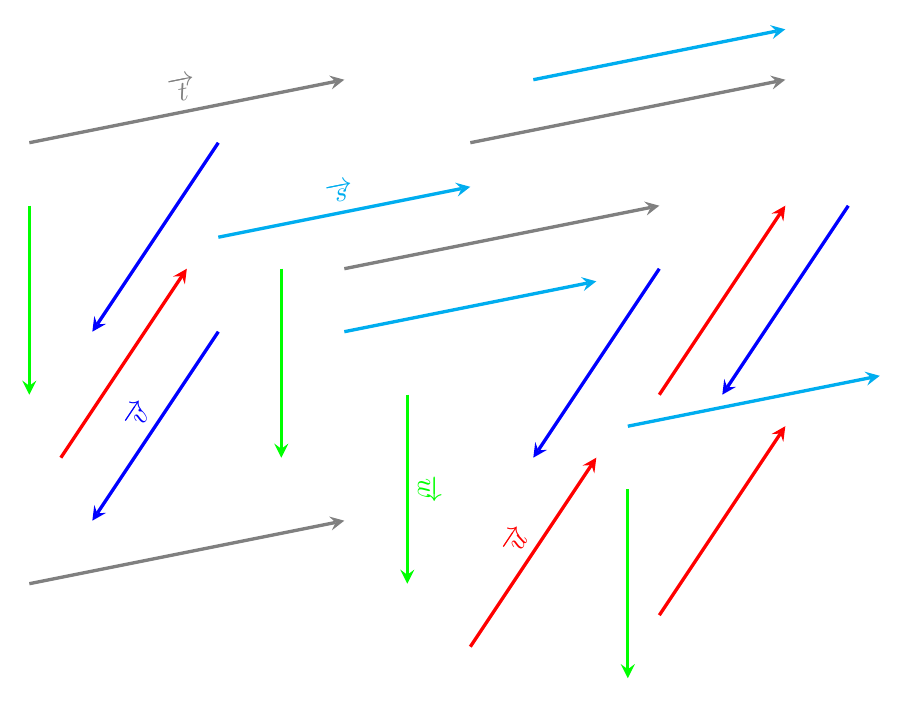
\begin{tikzpicture}[scale=0.8,every node/.style={scale=1}]
	\tikzstyle{vect}=[->,>=stealth,very thick]
	\tikzstyle{vectred}=[vect,red]
	\tikzstyle{vectblue}=[vect,blue]
	\tikzstyle{vectgreen}=[vect,green]
	\tikzstyle{vectgray}=[vect,gray]
	\tikzstyle{vectcyan}=[vect,cyan]
	

\coordinate (A) at (2,2);
\coordinate (B) at (5,6);
\coordinate (C) at (-4.5,5);
\coordinate (D) at (5,2.5);
\coordinate (u) at (2,3);
\draw[vectred] (A) -- ++ (u) node[midway, sloped, above]{$\overrightarrow{u}$};
\foreach \point in {B, C, D}
	\draw[vectred] (\point) -- ++ (u);

\coordinate (E) at (-2,7);
\coordinate (F) at (-2,10);
\coordinate (G) at (8,9);
\coordinate (H) at (5,8);
\coordinate (v) at (-2,-3);
\draw[vectblue] (E) -- ++ (v) node[midway, sloped, above]{$\overrightarrow{v}$};
\foreach \point in {F, G, H}
	\draw[vectblue] (\point) -- ++ (v);

\coordinate (I) at (1,6);
\coordinate (J) at (-1,8);
\coordinate (K) at (4.5,4.5);
\coordinate (L) at (-5,9);
\coordinate (w) at (0,-3);
\draw[vectgreen] (I) -- ++ (w) node[midway, sloped, above]{$\overrightarrow{w}$};
\foreach \point in {J, K, L}
	\draw[vectgreen] (\point) -- ++ (w);

\coordinate (M) at (-5,10);
\coordinate (N) at (-5,3);
\coordinate (O) at (0,8);
\coordinate (P) at (2,10);
\coordinate (t) at (5,1);
\draw[vectgray] (M) -- ++ (t) node[midway, sloped, above]{$\overrightarrow{t}$};
\foreach \point in {N, O, P}
	\draw[vectgray] (\point) -- ++ (t);

\coordinate (Q) at (-2,8.5);
\coordinate (R) at (4.5,5.5);
\coordinate (S) at (0,7);
\coordinate (T) at (3,11);
\coordinate (s) at (4,0.8);
\draw[vectcyan] (Q) -- ++ (s) node[midway, sloped, above]{$\overrightarrow{s}$};
\foreach \point in {R, S, T}
	\draw[vectcyan] (\point) -- ++ (s);
\end{tikzpicture}
\end{center}

\paragraph{Activité~3} Complétez les égalités suivantes~:\\
%\begin{center}
\begin{minipage}{0.5\textwidth}
\begin{tikzpicture}[scale=0.75,every node/.style={scale=1}]
	\tikzstyle{vect}=[->,>=stealth,ultra thick]
	
	\clip (-1,-1) rectangle (5,5);
	\placerpoint{A}{1}{2}{above left}
	\placerpoint{B}{2}{3}{above left}
	\placerpoint{C}{3}{2}{above right}
	\placerpoint{D}{2}{1}{below left}
	\draw (A) -- (B) -- (C) -- (D) -- cycle;
	\draw[vect] (A) -- (B);
	\draw[vect] (B) -- (C);
	\draw[vect] (A) -- (D);
	\draw[vect] (D) -- (C);
	\draw (0,0) grid (4,4);
\end{tikzpicture}
\end{minipage}
\begin{minipage}{0.5\textwidth}
\vectaffiche{AB} + \vectaffiche{BC} = \reponseEX{\vectaffiche{AC}} \\
\vectaffiche{AD} + \vectaffiche{DC} = \reponseEX{\vectaffiche{AC}}\\[1em]
\vectaffiche{AD} + \vectaffiche{CB} + \vectaffiche{AB} = \reponseEX{\vectaffiche{AB}}\\
\end{minipage}

\begin{minipage}{0.5\textwidth}
\begin{tikzpicture}[scale=0.75,every node/.style={scale=1}]
	\tikzstyle{vect}=[->,>=stealth,ultra thick]
	
	\placerpoint{E}{0}{2}{above left}
	\placerpoint{F}{2}{4}{above left}
	\placerpoint{G}{4}{2}{above right}
	\placerpoint{H}{2}{0}{below left}
	\draw (E) -- (F) -- (G) -- (H) -- cycle;
	\draw[vect] (E) -- (F);
	\draw[vect] (F) -- (G);
	\draw[vect] (E) -- (H);
	\draw[vect] (H) -- (G);
	\draw (-1,-1) grid (5,5);
\end{tikzpicture}
\end{minipage}
\begin{minipage}{0.5\textwidth}
\vectaffiche{EF} + \vectaffiche{FH} + \vectaffiche{HG} = \reponseEX{\vectaffiche{EG}} \\
\vectaffiche{EH} + \vectaffiche{HF} + \vectaffiche{FG} = \reponseEX{\vectaffiche{EG}} \\[1em]
\vectaffiche{EG} + \vectaffiche{FE} = \reponseEX{\vectaffiche{EH}} ( = \reponseEX{\vectaffiche{FG}} ) \\
\vectaffiche{EH} + \vectaffiche{EF} = \reponseEX{\vectaffiche{EG}} \\[1em]
\vectaffiche{FH} + \vectaffiche{EF} = \reponseEX{\vectaffiche{FG}} ( = \reponseEX{\vectaffiche{EH}} ) \\
\vectaffiche{GE} + \vectaffiche{FG} + \vectaffiche{EF} = \reponseEX{\vectaffiche{0}} \\[1em]
\end{minipage}



\vspace{-4em}


\end{minipage}
\newpage

\begin{minipage}{0.45\textwidth}
\thispagestyle{firststyle}

\vspace*{1em}


\paragraph{Activité~2} ~\\

%\section{Définitions}

%\vfill
\begin{center}
\begin{tikzpicture}[scale=0.8,every node/.style={scale=0.7}]
	\tikzstyle{vect}=[->,>=stealth,very thick]
%	\clip (0.1,0.1) rectangle (14.9,9.9);
	\placerpoint{O}{8}{7}{above left};
	\placerpoint{N}{10}{4}{below right};
	\grille{0}{0}{15}{10}{help lines};
	\vect{A}{B}{2}{4}{3}{8}{left}{right}{red};
%	\vect{C}{D}{4}{6}{4}{2}{above}{below}{red};
	\vect{C}{D}{11}{8}{14}{9}{left}{right}{red};
	\vect{E}{F}{14}{1}{12}{4}{right}{left}{red};
	\placerpoint{M}{7}{3}{left};
	\draw[vect,red,line width=1.5pt] (M) -- ++ (3,1);
	\draw[vect,red,line width=1.5pt] (M) ++ (3,1) -- ++ (-2,3);
	\draw[vect,<-,red,line width=1.5pt] (M) ++ (3,1) ++ (-2,3) -- (M);
%	\placerpoint{A}{5}{7}{left}
%	\placerpoint{B}{3}{4}{left}
\end{tikzpicture}
\end{center}

\begin{enumerate}
	\item Sur la figure ci-dessus, placer N image de M par la translation qui envoie C en D.
	\item Ensuite, placer O image de N par la translation qui envoie E en F.
	\item Que peut on dire de $\overrightarrow{AB}$ et de $\overrightarrow{MO}$~? \reponseEX{$\overrightarrow{AB}=\overrightarrow{MO}$}
	\item Quelle est la nature du quadrilatère ABOM~?\\ \reponseEX{C'est un parallélogramme}
\end{enumerate}
%\end{center}


%%%%%\begin{center}
%%%%%\begin{tikzpicture}[scale=0.8,every node/.style={scale=1}]
%%%%%	\tikzstyle{vect}=[->,>=stealth,very thick]
%%%%%	\tikzstyle{vectred}=[vect,red]
%%%%%	\tikzstyle{vectblue}=[vect,blue]
%%%%%	\tikzstyle{vectgreen}=[vect,green]
%%%%%	\tikzstyle{vectgray}=[vect,gray]
%%%%%	\tikzstyle{vectcyan}=[vect,cyan]
%%%%%	
%%%%%
%%%%%\coordinate (A) at (2,2);
%%%%%\coordinate (B) at (5,6);
%%%%%\coordinate (C) at (-4.5,5);
%%%%%\coordinate (D) at (5,2.5);
%%%%%\coordinate (u) at (2,3);
%%%%%\draw[vectred] (A) -- ++ (u) node[midway, sloped, above]{$\overrightarrow{u}$};
%%%%%\foreach \point in {B, C, D}
%%%%%	\draw[vectred] (\point) -- ++ (u);
%%%%%
%%%%%\coordinate (E) at (-2,7);
%%%%%\coordinate (F) at (-2,10);
%%%%%\coordinate (G) at (8,9);
%%%%%\coordinate (H) at (5,8);
%%%%%\coordinate (v) at (-2,-3);
%%%%%\draw[vectblue] (E) -- ++ (v) node[midway, sloped, above]{$\overrightarrow{v}$};
%%%%%\foreach \point in {F, G, H}
%%%%%	\draw[vectblue] (\point) -- ++ (v);
%%%%%
%%%%%\coordinate (I) at (1,6);
%%%%%\coordinate (J) at (-1,8);
%%%%%\coordinate (K) at (4.5,4.5);
%%%%%\coordinate (L) at (-5,9);
%%%%%\coordinate (w) at (0,-3);
%%%%%\draw[vectgreen] (I) -- ++ (w) node[midway, sloped, above]{$\overrightarrow{w}$};
%%%%%\foreach \point in {J, K, L}
%%%%%	\draw[vectgreen] (\point) -- ++ (w);
%%%%%
%%%%%\coordinate (M) at (-5,10);
%%%%%\coordinate (N) at (-5,3);
%%%%%\coordinate (O) at (0,8);
%%%%%\coordinate (P) at (2,10);
%%%%%\coordinate (t) at (5,1);
%%%%%\draw[vectgray] (M) -- ++ (t) node[midway, sloped, above]{$\overrightarrow{t}$};
%%%%%\foreach \point in {N, O, P}
%%%%%	\draw[vectgray] (\point) -- ++ (t);
%%%%%
%%%%%\coordinate (Q) at (-2,8.5);
%%%%%\coordinate (R) at (4.5,5.5);
%%%%%\coordinate (S) at (0,7);
%%%%%\coordinate (T) at (3,11);
%%%%%\coordinate (s) at (4,0.8);
%%%%%\draw[vectcyan] (Q) -- ++ (s) node[midway, sloped, above]{$\overrightarrow{s}$};
%%%%%\foreach \point in {R, S, T}
%%%%%	\draw[vectcyan] (\point) -- ++ (s);
%%%%%\end{tikzpicture}
%%%%%\end{center}
%%%%%
%%%%%\vspace{-2em}


%\vspace*{\stretch{1}}
%\centering
%\begin{tikzpicture}[scale=2,transform shape]
%\draw (0,0) \Fin;
%\draw (-1em,-1ex) -- (1em,-1ex);
%\path[scope fading=south] (-1em,-0.25em) rectangle (1em,-3.75ex);
%\draw[yscale=-1] (0,2ex) \Fin;
%\end{tikzpicture}
%\vspace*{\stretch{1}}


\end{minipage}
\end{document}
%
%
%\paragraph{Exercice~2} Propriétés des quadrilatères
%
%\begin{tikzpicture}[scale=1,every node/.style={scale=0.7}]
%\tikzstyle{debutfin}=[ellipse,draw,text=red]
%\tikzstyle{instruct}=[rectangle,draw,fill=yellow!50]
%\tikzstyle{test}=[diamond, aspect=6,thick,
%draw=blue,fill=yellow!50,text=blue]
%\tikzstyle{es}=[rectangle,draw,rounded corners=4pt,fill=blue!25]
%
%\node[debutfin] (debut) at (0,3) {Début};
%\node[es] (lire) at (0,2) {Prendre un quadrilatère $Q$};
%\node[test] (test) at (0,0) {Les diagonales ont-elles un milieu commun \ ?};
%%\node[instruct] (init) at (-2,2.5) {$S\leftarrow 0$};
%\node[instruct] (plus) at (0,-2.5) {$S\leftarrow S+N$};
%\node[instruct] (moins) at (0,-3.5) {$N\leftarrow N-1$};
%\node[es] (afficher) at (-4,-2) {Afficher la somme $S$};
%\node[debutfin] (fin) at (-4,-3) {Fin};
%
%\tikzstyle{suite}=[->,>=stealth,thick,rounded corners=4pt]
%\draw[suite](debut) -- (lire);
%\draw[suite](lire) -- (test.north);
%%\draw[suite](init) -- (test.north);
%\draw[suite](test.south) -- (plus);
%\draw[suite](plus) -- (moins);
%\draw[suite](test) -| (afficher);
%\draw[suite](afficher) -- (fin);
%\end{tikzpicture}
%
%
%%%%%\begin{tikzpicture}
%%%%%% définition des styles
%%%%%\tikzstyle{quadri}=[rectangle,draw,fill=yellow!50,text=blue]
%%%%%\tikzstyle{estun}=[->,>=latex,very thick,dotted]
%%%%%% les nœuds
%%%%%\node[quadri] (Q) at (0,3) {Quadrilatère};
%%%%%\node[quadri] (P) at (0,1.5) {Parallélogramme};
%%%%%\node[quadri] (R) at (-3,0) {Rectangle};
%%%%%\node[quadri] (L) at (3,0) {Losange};
%%%%%\node[quadri] (C) at (5,-1.5) {Carré};
%%%%%% les flèches
%%%%%\draw[estun] (P)--(Q);
%%%%%\draw[estun] (R)to[bend left](Q); \draw[estun] (R)--(P);
%%%%%\draw[estun] (L)--(Q.south east); \draw[estun] (L)--(P);
%%%%%\draw[estun] (C)to[bend right](Q.east); \draw[estun] (C)to[bend left](P);
%%%%%\draw[estun] (C)--(L.south east); \draw[estun] (C)to[bend left](R);
%%%%%% la légende
%%%%%\draw[estun] (-4.5,2.5)--(-3,2.5)node[midway,above]{est un};
%%%%%\end{tikzpicture}
